\chapter{Modelling}
	This chapter summarizes the problem and assumtions taken considering the pipeline following problem.
	A controller will be derived used for tracking and maneuvering of the AUV vehicle. A Kalman filter
	will be derived for the smothing and predictions of the pipeline and a guidance algorithm will be
	presented. Last, some basic behavior of the AUV to certain situations are threated. 


\section{Problem Outline}
\label{chap2:problem}
	To solve the pipeline following problem it is important to have a clear formulation of the problem.
	This is really a path following problem, since the pipeline can be represented as a continous path in
	space. The geometric convergence to the path is the primary objective. There can be dynamical
	constraints along the path, i.e velocity constraints but these are considered secondary to the goal of
	geometric convergence. When there are dynamic constraints the problem is a Trajectory Tracking
	Problem. If only geometric convergence are considered the problem is called a Path Following Problem.
	\cite{guidance-path-2d-3d}

	In this report the pipeline will be formulated as a two dimentional path. This because the pipeline
	are layed on the sea bottom, and are assumed to follow the bottom signature. Then the path following
	are reduced to a two dimentional problem and the \textit{heave} state can be decoupled and in the
	controller design. The depth controller then needs to keep a constant height above the sea bottom.

	In order to limit the problem and ease the implementation, the pipeline are assumed to be a stright or
	nearly strigth, peice-wise continous line segment. The pipeline can only change direction at defined
	places called junctions. The application of this guidance system are only for long, continous streches of
	piplines. 

	An AUV carrying out a pipeline inspection mission is in most cases a low speed assumtion is valid. The
	\textit{HUGIN 1000} AUV are designed for speeds from 0-3 m/s. The inspection speed assumed in the
	rest of the report are around 1 m/s. This are realtively low speed, and the quadratic terms in the
	Coriolis/centripetal or Damping matices can be neglected. Later simulations verify this assumtion.

	\begin{figure}[hbtp]
		\centering
		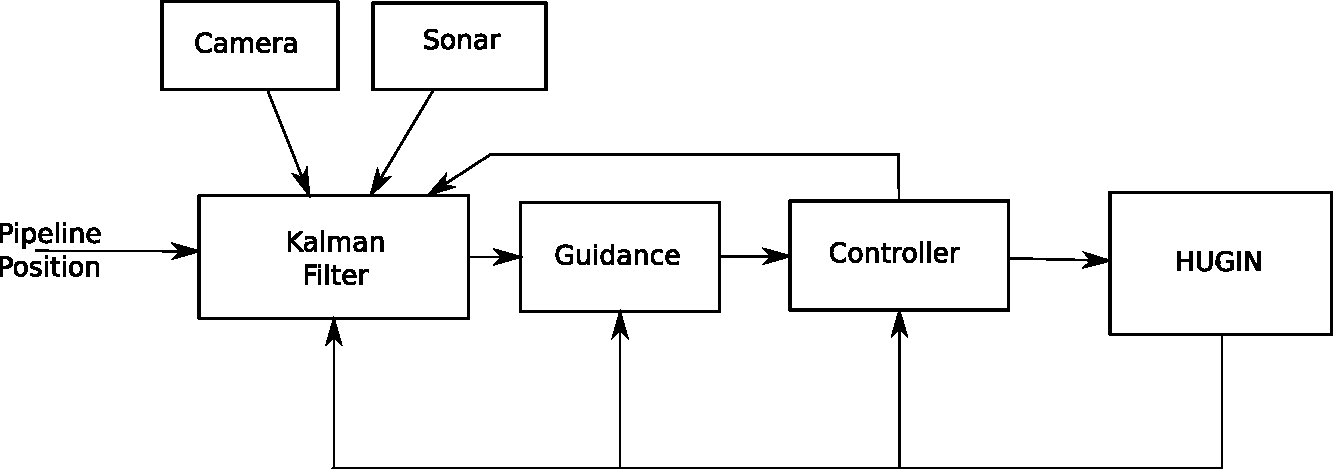
\includegraphics[width=0.9\textwidth]{pics/blockdiagram}
		\caption{Block diagram the path following controller}
		\label{fig:ch2-blockdiagram}
	\end{figure}
	As outlined in Figure \ref{fig:ch2-blockdiagram} the building stones of the  pipeline following
	control system are the control system are the cruising controller, guidance system and the filter
	which fuses the known data about the pipeline and the measured pipeline data. To recreate the 
	pipeline coordinates in three dimentions the distance to the sea bottom is measured by a sonar. The
	filter uses prior knowledge about the pipeline to-be-followd which can be inaccurate. The filter then
	uses this together with the altitude information and camera output to estimate the position of the
	pipeline. If the pipeline should be lost at any time the filter will try to predict where the pipeline
	are and serve as input to the guidance system.

	The system should be able to handle sections where the pipeline are burried and not visible to the
	camera. To too some extent eliminate this problem other sensors can be included to which uses other
	sensing methods than vision. Suiting sensors are magnetic anomalities sensors which can detect
	ferretic alloys and materials. Multi-beam echosounders and side scan sonar are other possible sensors
	to help detecting a burried pipeline.

\section{Controller Design}
	The model discussed in Section \ref{sec:ch1-model} is used to derive the controller equations for the
	AUV control system.

	The control system which supply the lower-level control system with forces and moments references, is 
	divided into 3 sub systems:
		\begin{itemize}
			\item Speed control
			\item Depth control
			\item Heading control
		\end{itemize}
	This is called the flightmode controller, which is used for normal pipeline tracking, descent and
	ascent. This type of controller where chosen because it will be more energy efficient than other more
	actuated controllers. The second reason is even if the AUV is almost fully actuated, i.e
	controllable in 5 DOF, the tunnel thrusters which have to be present for this degree of actuation are almost
	usless for higher velocities. This renders just control in 3 DOF, \textit{surge, pitch} and
	\textit{yaw}. This will give the most energy efficient pipeline following. 
	
	The \textit{HUGIN}-type AUV is a slender-body type AUV. This makes it possible to neglect the some
	coupling effects in between the states in the dynamic model. This means that one can decopuple the
	\textit{longitudinal} states (\textit{surge, heave, pitch}) from the \textit{lateral} states 
	(\textit{sway, roll, yaw}).

	The goal of the AUV is to inspect pipelines. This includes get good pictures of the pipeline for
	inspection by a human opperator. Since the AUV might be affected by ocean currents and might drift of
	the pipeline, it is convenient to define a over the pipeline controller whose goal is to keep the
	vessel directly over the pipeline. 

	All coefficient next are defined in accordance with \cite{SNAME}.
	\subsection{Speed Controller}
		The speed controller is derived form the \textit{surge}-subsystem, called \textit{surge}-model
		\cite{fossen}. Under the slow speed assumption, the coriolis/centripetal-matrix is assumed
		zero, $\coriolis \approx 0$  
		\begin{equation}
			(m - X_{\dot{u}})\dot{u} - X_u u - X_{|u|u}|u| u = \tau_1
		\end{equation}
		Setting $\tau_1 = -K_p \tilde{u} - K_i \int \tilde{u} dt - K_d \dot{u}$ the error in the velocity
		reference will go to zeros. The velocity reference is assumed constant and the PID controller
		guarantees that the error will go to zero.
	
	
	
	\subsection{Depth Controller}
		To derive the depth controller in the crusing control system the
		\textit{longitudinal}-subsystem is used as the control model \cite{fossen}. By assuming that the lateral
		states are small, i.e $v, p, r, \phi$, the kinematics can be derived as follows:
		\begin{equation}
			\left [ \begin{matrix}
					\dot{d} \\
					\dot{\theta}
				\end{matrix} \right] = \left [ \begin{matrix}
								\cos{\theta} & 0 \\
								0 & 1
								\end{matrix} \right] 
						\left[ \begin{matrix}
								w \\
								q
							\end{matrix} \right]
						+ \left [ \begin{matrix}
								-\sin{\theta}\\
								0
							\end{matrix} \right] u
		\end{equation}
		The dynamics of the system then becomes
		\begin{equation}
			\begin{aligned}
				\left [ \begin{array}{ccc}
					m - X_{\dot{u}} &  X_{\dot{w}} & m z_g - X_{\dot{q}} \\
					X_{\dot{w}} & m - Z_{\dot{w}} & m x_g - Z_{\dot{q}} \\
					m z_g - X_{\dot{q}} & m x_g - Z_{\dot{q}} & I_y - M_{\dot{q}} 
					\end{array} \right]
				\left [ \begin{array}{c}
					\dot{u} \\
					\dot{w} \\
					\dot{q} 
					\end{array} \right] \\
				+ \left [ \begin{array}{ccc}
					-X_u	&	-X_w 	&	-X_q \\
					-Z_u	&	-Z_w	&	-Z_q \\
					-M_u	&	-M_w	&	-M_q
					\end{array} \right]
				\left [ \begin{array}{c}
					u \\
					w \\
					q 
				\end{array} \right] + 
				\left [ \begin{array}{ccc} 
					0 & 0 & 0 \\
					0 & 0 &  -(m - X_{\dot{u}}) u \\
					0 & (Z_{\dot{w}} - X_{\dot{u}}) u & m x_g u 
					\end{array} \right]	
				\left [ \begin{array}{c}
					u \\
					w \\
					q 
				\end{array} \right] \\
				+  \left [ \begin{array}{c}
					0 \\
					0 \\
					W z_b \sin \theta \\
					\end{array} \right] = \left [ \begin{array}{c}
									\tau_1 \\
									\tau_3 \\
									\tau_5
								      \end{array} \right ]
			\end{aligned}
		\end{equation}
		Since the \textit{surge}-speed are stabilized with the controller derived in the previous
		section, the surge equation can be removed from the system under the assumption $u = u_0$.		
		Also by asuming that the \textit{heave}-velocity and $\theta$ are small the control model
		becomes:
		\begin{equation}
			\left [ \begin{matrix}
					\dot{d} \\
					\dot{\theta} \\
					\dot{q} 
				\end{matrix}
				\right ] = \left [ \begin{matrix}
							0 & -u_0 &  0 \\
							0 & 0 &   1 \\
							0 & -\frac{1}{\gamma} W &-\frac{1}{\gamma}M_{w} 
							(m - Z_{\dot{w}})-M_w Z_q
						\end{matrix} \right ] 
				\left [ \begin{matrix}
						d \\
						\theta \\
						q
					\end{matrix} \right] + \left [ \begin{matrix}
										0 \\
										0 \\
										\frac{1}{\gamma}
									\end{matrix} \right] \tau_5
		\end{equation}
		where $\gamma = m I_y - m M_{\dot{q}} - I_y Z_{\dot{w}} + Z_{\dot{w}} M_{\dot{q}}$.
		
		When closing the loop the following is proposed PID-like controller
		\begin{equation}
			\begin{aligned}
				\tau_5 &= -K_{dp} \tilde{d} + K_{dd}  \theta + K_{dd2} q \\
				\tilde{d} &= d - d_d \quad \dot{\tilde{d}} = -u_0\theta \quad
				\ddot{\tilde{d}} = -u_0q
			\end{aligned}
		\end{equation}
		A similiar controller are implemnted in \cite{NDRE-AUV}.
				

	
	\subsection{Heading Controller}
		Using the \textit{lateral}-subsystem representation from \cite{fossen}. Under the assumtions
		that $w, p, q, r, \phi,$ and $\theta$ from the longitudinal subsystem are small, the
		kinematics are reduced to:
		\begin{align}
			\dot{\phi} &= p \\
			\dot{\psi} &= r 
		\end{align}
		The low-speed assumtion is utilized, higher order velocity terms are neglected, and
		constant \textit{surge}-velocity $u = u_0$ are| assumed. This gives the following system:
		\begin{equation}
			\begin{aligned}
				\left [ \begin{array}{ccc}
					m - Y_{\dot{v}} & - m z_g - Y_{\dot{p}} & m x_g - Y_{\dot{r}} \\
					-m z_g - Y_{\dot{p}} & I_x - K_{\dot{p}} & I_{zx} - K_{\dot{r}} \\
					m x_g - Y_{\dot{r}} & I_{zg} - K_{\dot{r}} & I_z - N_{\dot{r}} 
					\end{array} \right]
				\left [ \begin{array}{c}
					\dot{v} \\
					\dot{p} \\
					\dot{r} 
					\end{array} \right] \\
				+ \left [ \begin{array}{ccc}
					-Y_v	&	-Y_p 	&	-Y_r \\
					-M_v	&	-M_p	&	-M_r \\
					-N_v	&	-N_P	&	-N_r
					\end{array} \right]
				\left [ \begin{array}{c}
					v \\
					p \\
					r 
				\end{array} \right] + 
				\left [ \begin{array}{ccc} 
					0 & 0 & (m - X_{\dot{u}})u \\
					0 & 0 &  0 \\
					(X_{\dot{u}} - Y_{\dot{v}}) u & 0 & m x_g u 
					\end{array} \right]	
				\left [ \begin{array}{c}
					v \\
					p \\
					r 
				\end{array} \right] \\
				+  \left [ \begin{array}{c}
					0 \\
					W z_b \sin \phi \\
					0 
					\end{array} \right] = \left [ \begin{array}{c}
									\tau_2 \\
									\tau_4 \\
									\tau_6
								      \end{array} \right ]
			\end{aligned}
		\end{equation}
		The \textit{roll}-state can be removed from the equations because of the assumtions of small
		$\dot{p}, p$ and that the \textit{sway}-velocity can be neglected, the sway subsystem can be
		removed as well. This can be done because the vessel are considered stabel in roll because of
		the offset in the bouyancy point. This can be seen from the simulations later in the report as
		well. 

		The following control model are used to derive the heading controller. The model is really
		the 1st order Nomoto model, and have become famous for it simplicity yet prove to give good
		results. 
		\begin{equation}
			\left [ \begin{matrix}
					\dot{\psi} \\
					\dot{r}
				\end{matrix} \right]  =  \left [ \begin{matrix}
								0 & 1 \\
								0 & \frac{N_r - m x_g u_0}{I_z - N_{\dot{r}}}\\
								\end{matrix} \right] 
							\left [ \begin{matrix}
									\psi \\
									r
								\end{matrix} \right]
							+ \left [ \begin{matrix}
									0\\
									\frac{1}{I_z - N_{\dot{r}}}
								\end{matrix} \right] \tau_6
		\end{equation}

		The following heading controller are proposed:
		\begin{equation}
			\tau_6 = T\dot{r_d} + r_d - K_{hp} \tilde{\psi} - K_{hi} \int \tilde{\psi} dt - K_{hd}
			\dot{\tilde{\psi}}
		\end{equation}
		The terms $T \dot{r_d} + r_d$ are reference feed forward terms which will guarantee perfect
		tracking during course-changing maneuvers according to \cite{fossen}. 

	
	\subsection{Over-Pipeline Tracking Controller}
		When the AUV is over the pipeline the need to keep the AUV on top of the pipeline to get deecent 
		pictures for the pipeline inspection, presents itself. To solve this problem a second controller 
		have been created just for this purpose. Since the vessel is controllable in 5 DOF the ability to 
		create a good controller for this purpose is good. 
		
		The controller uses input form the camera to get the position of the AUV relative to the pipeline 
		and give a suitable input to the controller.




\section{Pipeline representation}
	The representation of the pipeline is important because it is used in the Kalman filter to predict
	where the pipeline is going. The pipeline is parametrized by $\varpi \in \mathbb{R}$ to get a
	continous and smooth pipeline.

	In this report the pipeline are parameterized as:
	\begin{equation}
		P_w(\varpi) = \left [ \begin{array}{c}
					\varpi \\
					k_y \varpi \\
					z(\eta)
				\end{array} \right ] \quad \varpi \in (0, \infty)
	\end{equation}
	where $k_y$ are constant and $z(\eta)$ is some function described by the sea bottom and are assumed
	known. 
	
	


\section{Kalman filter}
	The Kalman filters purpose is to smooth the camera output and predict forward where the pipeline will
	be in the future to supply a better heading reference for the guidance controller.

	The position of the pipeline are given some uncertanty becuase the pipeline may have moved after it
	was layed or the position might be erronous. This gives:
	\begin{equation}
		P_w(\varpi) = \left [ \begin{array}{c}
					\varpi \\
					k_y \varpi \\
					z(\eta)
				\end{array} \right ] + \mathbf{B}\delta
	\end{equation}
	The function $\delta$ are a slowly varying disturbance which can be modeled as a \textit{1st order Markov
	Process}, and $\mathbf{B}$ is some 2x3 matrix.
	\begin{equation}
		\dot{\delta} = -\mathbf{T} \delta +  w
	\end{equation}
	where $w \in \mathbb{R}^2$, are a zero mean unity variance white noise process. This describes the
	error in the position. The matrix $\mathbf{T}$ specifies how the error evolves. Time differentianting
	the position estimate with regard to time gives
	\begin{equation}
		\dot{P_w}(\varpi) =  \left [ \begin{array}{c}
						\dot{\varpi} \\
						k_y \dot{\varpi} \\
						\dot{z}(\eta)
					\end{array} \right ] + \dot{\delta}
	\end{equation}
	By setting $\varpi = N(t)$, i.e the North position and completely disregarding the depth coordinate.
	gives the following
	\begin{equation}
		\dot{P_w'} = \left [ \begin{array}{c}
					n \\
					k_y n 
				\end{array} \right ] + \dot{\delta}
	\end{equation}
	Choseing the state vector and input as:
	\begin{equation}
		x = [ P_w'^T \quad \delta^T]^T \quad \Rightarrow  \quad \dot{x} = [\dot{P_w'^T} \quad
		\dot{\delta^T}]^T \quad  u = n
	\end{equation}
	This calls for the following state space representation 
	\begin{equation}
		\dot{x} = \left [ \begin{array}{cc}
					0 & -T \\
					0 & -T
				\end{array} \right] x + \left [ \begin{array}{c}
								1 \\
								k_y\\
								0 \\
								0
								\end{array} \right] u +
				\left [ \begin{array}{c}
						\mathbf{0}_{2x2} \\
						\mathbf{I}_{2x2} 
					\end{array} \right] w
	\end{equation}

	The measurement model are more complex. To be able to compare the measurement from the camera with the
	state space model, the perspective equations from Section \ref{ch1-cameramodel} are needed. By using
	Equations \eqref{eq:ch1-P_c} and \eqref{eq:ch1-perspective}, we can transform the point from World
	coordinates to image coordinates. We want $y = P_i$
	\begin{equation*}
		y = P_i = \mathbf{H} P_c = \mathbf{H R}^T ( P_w - O(t))
	\end{equation*}
	$O(t)$ is the origin of the camera frame and is equal to the position vector $\eta' = [N(t),
	E(t)]^T$ of the AUV in the NED frame. By including the position vector in the input to the filter and using 
	$P_w = \mathbf{C} x$, the measurement model are conclueded.
	\begin{equation}
		\label{eq:ch2-measurement}
		y = \mathbf{H R}^T \mathbf{C} x - \mathbf{H R}^T  O(t) = \mathbf{C}'x + \mathbf{D} u
	\end{equation}
	where $\mathbf{C'}$ and $\mathbf{D}$ are apropriate matrices for selecting the right states. $\mathbf{R}$
	are the Rotation Matrix from World coordinates to Camera coordinates. This gives the following model
	for the Kalman filter
	\begin{align}
		x &= \mathbf{A} x + \mathbf{B} u + \mathbf{E} w\\
		y &= \mathbf{C}'x + \mathbf{D} u + v\\
		\mathbf{A} &= \left [ \begin{matrix}
					0 & 0 & -T_1 & 0 \\
					0 & 0 & 0 & -T_2 \\
					0 & 0 & -T_1 & 0 \\
					0 & 0 & 0 & -T_2 
					\end{matrix} \right] \quad \mathbf{B} = \left[ \begin{matrix}
										1 & 0 & 0 \\
										k_y & 0 & 0\\
										0   & 0 & 0 \\
										0 & 0 & 0
										\end{matrix} \right]\\
		\mathbf{E} &= \left [ \begin{matrix}
					0 & 0 \\
					0 & 0 \\
					1 & 0 \\
					0 & 1
					\end{matrix} \right] \quad \mathbf{C}' = \left [ \begin{matrix}
						\frac{f}{z_c} \cos{\psi} &\frac{f}{z_c} \sin{\psi} & 0 & 0 \\
						-\frac{f}{z_c} \sin{\psi}& \frac{f}{z_c} \cos{\psi} & 0 & 0 
								\end{matrix} \right] \\
		\mathbf{D} &= \left [ \begin{matrix}
					0 & -\frac{f}{z_c} \cos{\psi} & -\frac{f}{z_c} \sin{\psi} \\
					0 & \frac{f}{z_c} \sin{\psi} & -\frac{f}{z_c} \cos{\psi}
					\end{matrix} \right]
	\end{align}
	$w, v$ are a vectors of unity white noise and have covariance $E(ww^T) = \mathbf{Q}$ and $E(vv^T) =
	\mathbf{W}$


\section{Summary of Assumtions}
	A summary of the assumtions are given here:
	\begin{enumerate}
		\item The pipeline is layed on the sea bottom, which gives the pipeline the same
		height signature as the sea bottom. The guidance problem is then reduced to a
		two-dimentional problem.
		\item Pitch- and roll angles, are assumed small together with the corresponding pitch- and
		roll rates. In the vicinity of $\pm 5^{\circ}$ and $\pm 0.05 \mathrm{rad/s}$
		\item \textit{sway} and \textit{heave} velocities are small compared to \textit{surge}
		velocity and any cross-coupling terms may be neglected.
		\item The full state are assumed perfectly known. 
		\item The exact position of the are known.
	\end{enumerate}
		
\section{Guidance system}
	The guidance block are one of the most important building stones of an Autonomous system. It needs
	some guidance for what it needs to do. Figure \ref{fig:ch2-Guidance-block} shows a proposal of a
	guidance and descision system for the \textit{HUGIN} vehicle.
	\begin{figure}[htbp]
		\centering
		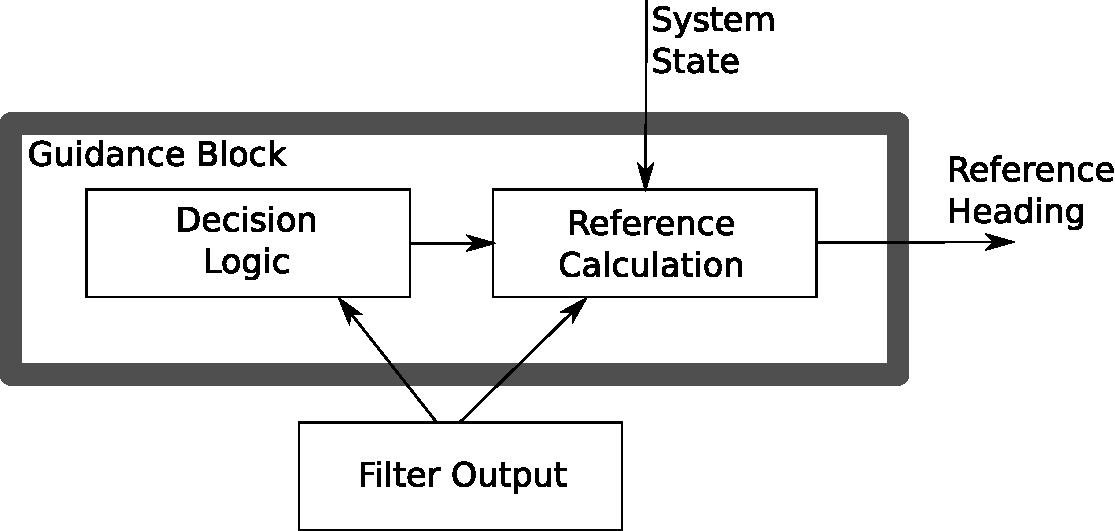
\includegraphics[width=0.8\textwidth]{pics/guidance}
		\caption{Guidance System Block}
		\label{fig:ch2-Guidance-block}
	\end{figure}

	The AUV control system are assumed to have three modes, \textit{searching}, \textit{tracking} and
	\textit{initialize/finalize}. The \textit{initialize/finalize}-mode are the beginning and end of a
	mission and will not be considered in this report. 
	
	The \textit{searching}-mode are when the AUV are looking for the pipeline. When the pipeline are layed
	on the sea floor, the position may be more or less inexact. Both because of sometimes the great 
	distance from the sea level and to the sea bottom, and sometimes because the pipeline have ``sagged'', 
	i.e moved away from the initial position because of movement in the sea bottom. In most cases the
	pipeline will not have moved that much away from the inital position. 
	\begin{figure}[htbp]
		\centering
		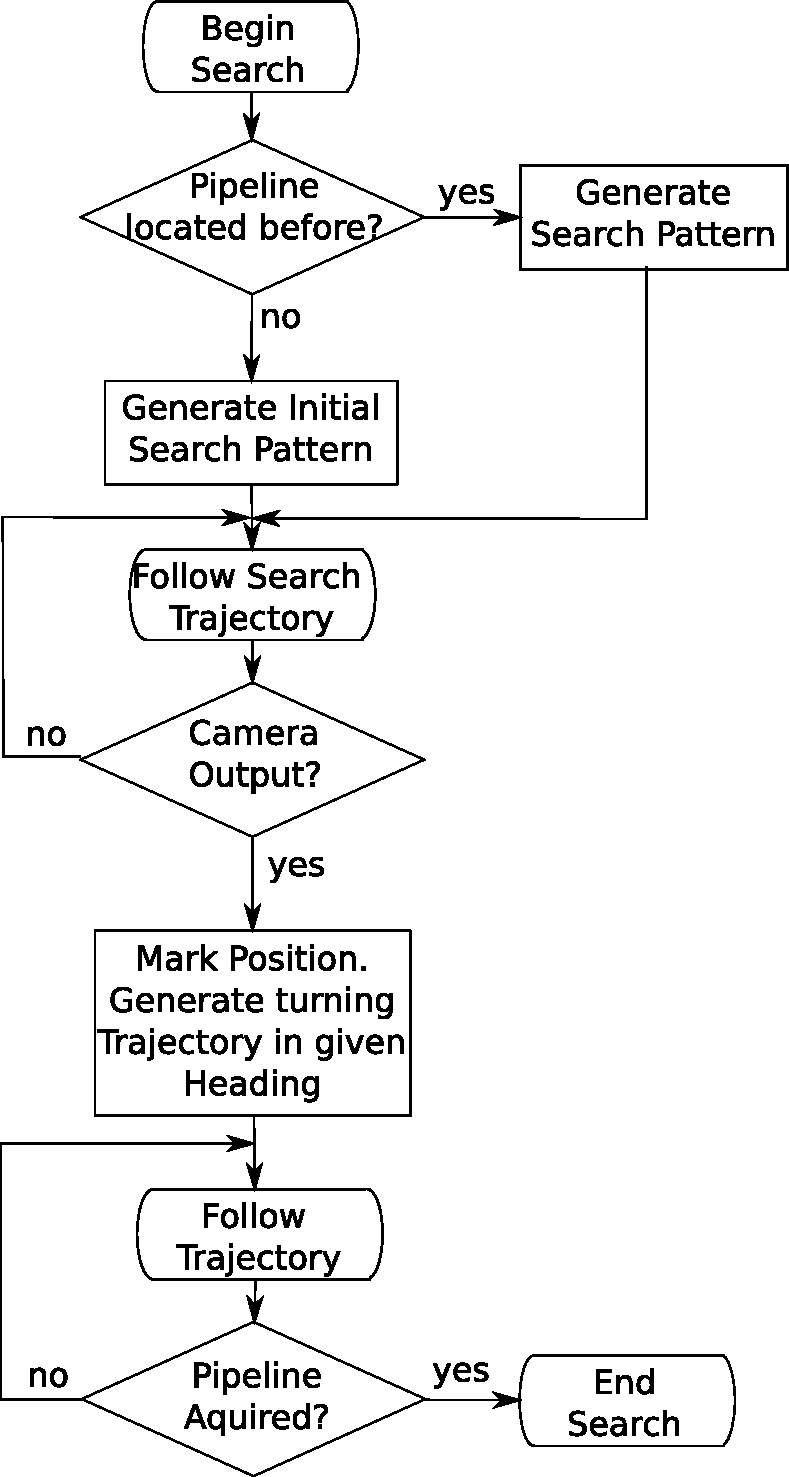
\includegraphics[width=0.5\textwidth]{pics/search_flow}
		\caption{Flow diagram of the search procedure in the \textit{searching}-mode}
		\label{fig:ch2-search-flow}
	\end{figure}

	***************************

	The search procedure will be different depending on if it is the initial acquisition or reacquisition.
	If inital acquisition, the area that have to be searched are greater than the search area for
	reacquisition.


	\subsection{Decision Logic}
		The descision block of the guidance system needs to deal with problems that arise under a
		pipeline inspcetion mission, such as when the pipeline are lost from the camera field-of-view.
		What is the apropriate action? When should it start searching for the pipeline? 

		The idea is that the pipeline should not be able to take sudden turns. There are limited
		curvature, i.e the pipeline can only turn so much, over a limited distance. The posibility of
		pipeline junctions are not considered. The assumtion is that the pipeline are a long continous
		straight segment. If the pipeline is lost the filter will continue to predict where the
		pipeline should have been. The AUV follows the predicted path for some time. If the pipeline
		are not reaquired after that time, the AUV have to go back to the pipelines last known
		position, and start some search pattern.

		
	

	\subsection{Reference Calculation}
		A look-ahead based guidance algorithm is chosen for it's simplicity and robustness. All
		together a pipeline are made up of mostly linear segments, and the general direction of the
		pipeline are knonw to be very exact. This algoritms should provide good results and keep 
		the cross-track error to a minimum.

		In the presence of ocean current it will cause the heading to ``lean'' towards the current if
		the look-ahead distance is not chosen too far away. 
		
	
	\subsection{Search Patterns}
		\label{subsec:ch2_searchpattern}
		It is obvious that some kind of search pattern must be implemented for this kind of
		application. This might be customized for every mission or it might be selected from a library
		of suiting search patterns. 
		This section will look at some search patterns which might be suiting for the pipeline search
		application.

		\begin{figure}[htbp]
			\centering
			\subfigure[Divergent Zig-Zag pattern for lost pipeline during tracking]{
				\label{fig:ch2_zig_zag}
				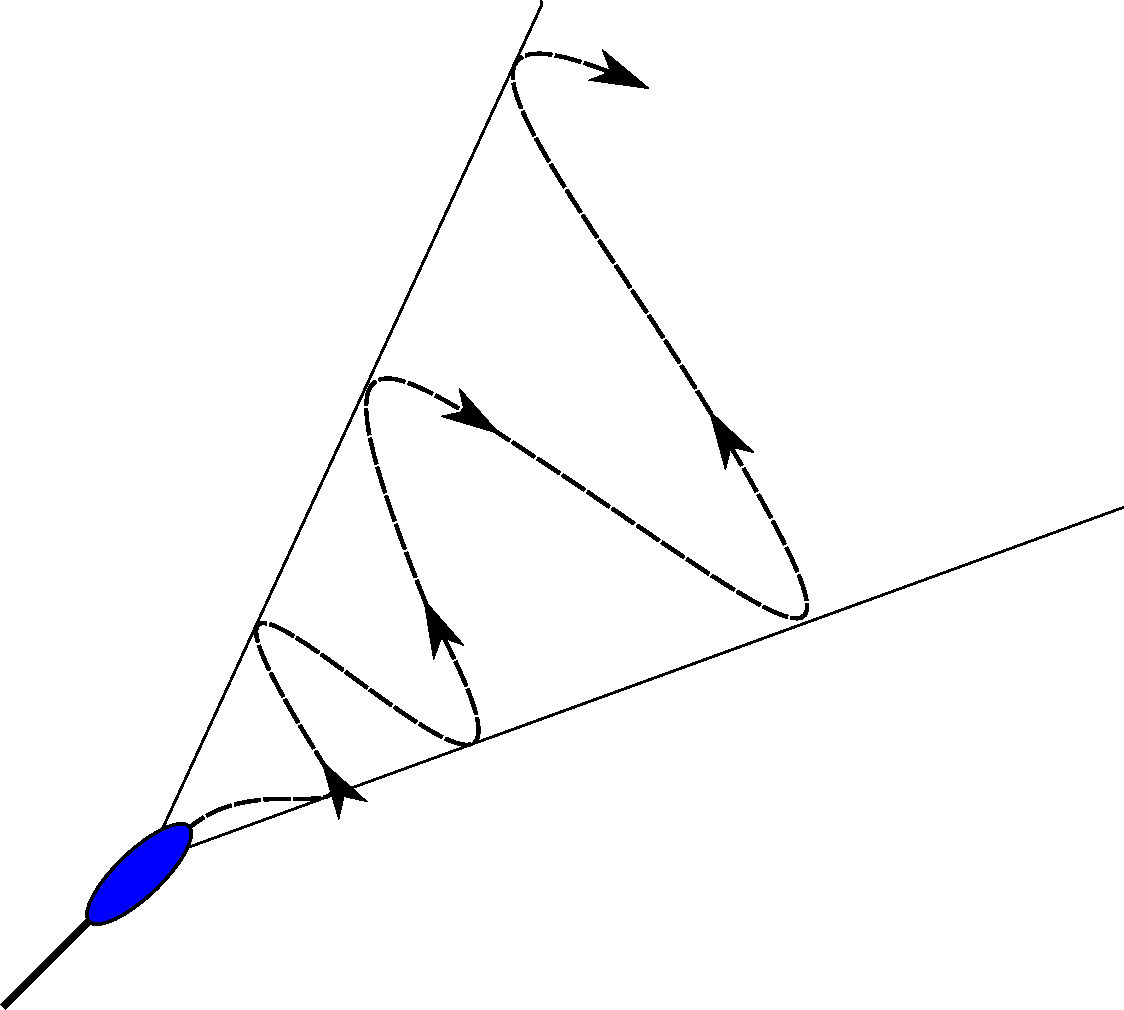
\includegraphics[width=0.4\textwidth]{pics/divergent_zig-zag}} \quad
			\subfigure[Outwards spiral pattern for inital pipeline search]{
				\label{fig:ch2_spiral}
				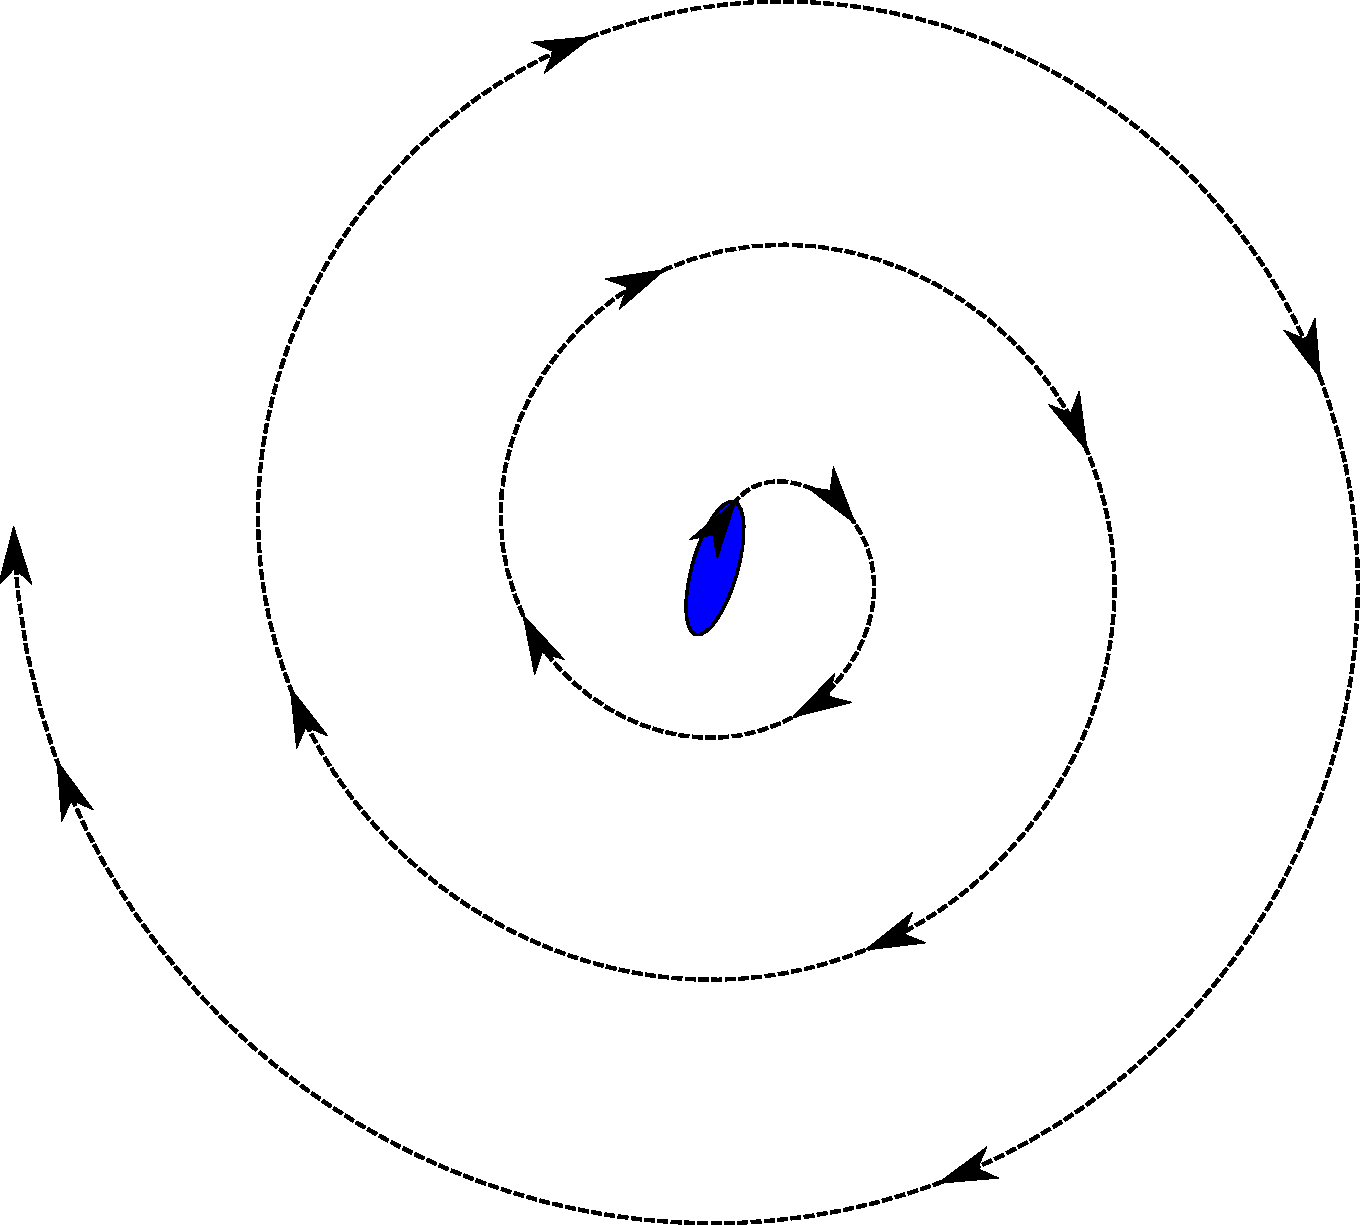
\includegraphics[width=0.4\textwidth]{pics/spiral_search}}
			\caption{Differnet search pattern}
			\label{fig:ch2_searchpattern}
		\end{figure}
		The first case is when the pipeline are not in its predetermined position or the position
		sensors gives out erronous readings, some kind of search need to be initiated to find the
		pipeline. This could be something like the depicted case in Figure~\ref{fig:ch2_spiral}.
		Spiral pattern going outwards to try to find the pipeline in the visinity of the AUV position.
		This should be aided with other sensors for example with a Side Scan Sonar which provides good
		sensor data in the horizontal directions around the AUV. 

		The other case is when the pipeline are lost during tracking. Since the general direction of
		the pipeline are assumed known, the other pattern are a divergent zig-zag pattern around the
		assumed pipeline trajectory, from the last known position. This should work well to reacuire
		the pipeline after loosing it.
		
	
\section{Overall System}
	The system flow are depicted in Figure~\ref{fig:ch2-flowdiagram}. This is how the overall system behaves
	during a pipeline inspection mission. 
	\begin{figure}[htbp]
		\centering
		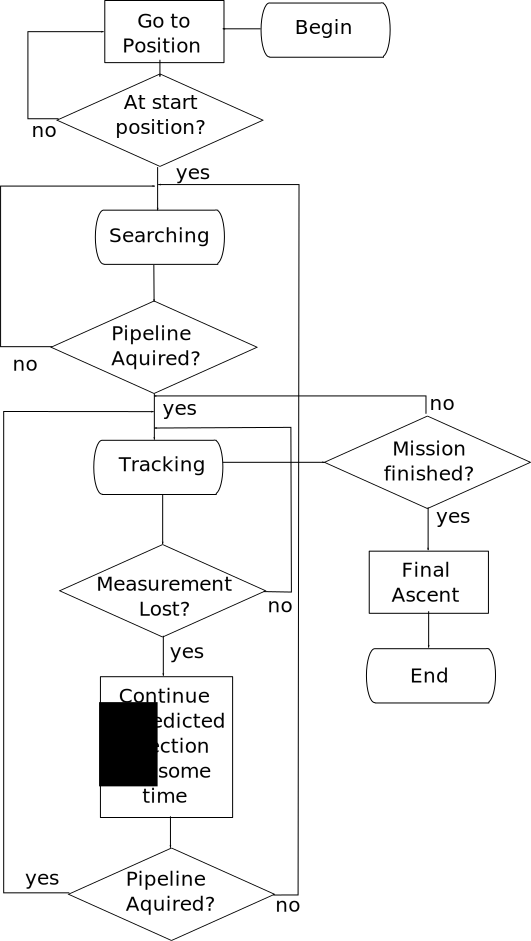
\includegraphics[width=0.5\textwidth]{pics/Operation}
		\caption{Flow diagram of pipeline inspection mission}
		\label{fig:ch2-flowdiagram}
	\end{figure}
	
	

